\documentclass[journal,12pt,twocolumn]{IEEEtran}

\usepackage{setspace}
\usepackage{gensymb}

\singlespacing


\usepackage[cmex10]{amsmath}

\usepackage{amsthm}

\usepackage{mathrsfs}
\usepackage{txfonts}
\usepackage{stfloats}
\usepackage{bm}
\usepackage{cite}
\usepackage{cases}
\usepackage{subfig}

\usepackage{longtable}
\usepackage{multirow}

\usepackage{enumitem}
\usepackage{mathtools}
\usepackage{steinmetz}
\usepackage{tikz}
\usepackage{circuitikz}
\usepackage{verbatim}
\usepackage{tfrupee}
\usepackage[breaklinks=true]{hyperref}

\usepackage{tkz-euclide}

\usetikzlibrary{calc,math}
\usepackage{listings}
    \usepackage{color}                                            %%
    \usepackage{array}                                            %%
    \usepackage{longtable}                                        %%
    \usepackage{calc}                                             %%
    \usepackage{multirow}                                         %%
    \usepackage{hhline}                                           %%
    \usepackage{ifthen}                                           %%
    \usepackage{lscape}     
\usepackage{multicol}
\usepackage{chngcntr}

\DeclareMathOperator*{\Res}{Res}

\renewcommand\thesection{\arabic{section}}
\renewcommand\thesubsection{\thesection.\arabic{subsection}}
\renewcommand\thesubsubsection{\thesubsection.\arabic{subsubsection}}

\renewcommand\thesectiondis{\arabic{section}}
\renewcommand\thesubsectiondis{\thesectiondis.\arabic{subsection}}
\renewcommand\thesubsubsectiondis{\thesubsectiondis.\arabic{subsubsection}}


\hyphenation{op-tical net-works semi-conduc-tor}
\def\inputGnumericTable{}                                 %%

\lstset{
%language=C,
frame=single, 
breaklines=true,
columns=fullflexible
}
\begin{document}


\newtheorem{theorem}{Theorem}[section]
\newtheorem{problem}{Problem}
\newtheorem{proposition}{Proposition}[section]
\newtheorem{lemma}{Lemma}[section]
\newtheorem{corollary}[theorem]{Corollary}
\newtheorem{example}{Example}[section]
\newtheorem{definition}[problem]{Definition}

\newcommand{\BEQA}{\begin{eqnarray}}
\newcommand{\EEQA}{\end{eqnarray}}
\newcommand{\define}{\stackrel{\triangle}{=}}
\bibliographystyle{IEEEtran}
\providecommand{\mbf}{\mathbf}
\providecommand{\pr}[1]{\ensuremath{\Pr\left(#1\right)}}
\providecommand{\qfunc}[1]{\ensuremath{Q\left(#1\right)}}
\providecommand{\sbrak}[1]{\ensuremath{{}\left[#1\right]}}
\providecommand{\lsbrak}[1]{\ensuremath{{}\left[#1\right.}}
\providecommand{\rsbrak}[1]{\ensuremath{{}\left.#1\right]}}
\providecommand{\brak}[1]{\ensuremath{\left(#1\right)}}
\providecommand{\lbrak}[1]{\ensuremath{\left(#1\right.}}
\providecommand{\rbrak}[1]{\ensuremath{\left.#1\right)}}
\providecommand{\cbrak}[1]{\ensuremath{\left\{#1\right\}}}
\providecommand{\lcbrak}[1]{\ensuremath{\left\{#1\right.}}
\providecommand{\rcbrak}[1]{\ensuremath{\left.#1\right\}}}
\theoremstyle{remark}
\newtheorem{rem}{Remark}
\newcommand{\sgn}{\mathop{\mathrm{sgn}}}
\providecommand{\abs}[1]{\left\vert#1\right\vert}
\providecommand{\res}[1]{\Res\displaylimits_{#1}} 
\providecommand{\norm}[1]{\left\lVert#1\right\rVert}
%\providecommand{\norm}[1]{\lVert#1\rVert}
\providecommand{\mtx}[1]{\mathbf{#1}}
\providecommand{\mean}[1]{E\left[ #1 \right]}
\providecommand{\fourier}{\overset{\mathcal{F}}{ \rightleftharpoons}}
%\providecommand{\hilbert}{\overset{\mathcal{H}}{ \rightleftharpoons}}
\providecommand{\system}{\overset{\mathcal{H}}{ \longleftrightarrow}}
	%\newcommand{\solution}[2]{\textbf{Solution:}{#1}}
\newcommand{\solution}{\noindent \textbf{Solution: }}
\newcommand{\cosec}{\,\text{cosec}\,}
\providecommand{\dec}[2]{\ensuremath{\overset{#1}{\underset{#2}{\gtrless}}}}
\newcommand{\myvec}[1]{\ensuremath{\begin{pmatrix}#1\end{pmatrix}}}
\newcommand{\mydet}[1]{\ensuremath{\begin{vmatrix}#1\end{vmatrix}}}
\numberwithin{equation}{subsection}
\makeatletter
\@addtoreset{figure}{problem}
\makeatother
\let\StandardTheFigure\thefigure
\let\vec\mathbf
\renewcommand{\thefigure}{\theproblem}
\def\putbox#1#2#3{\makebox[0in][l]{\makebox[#1][l]{}\raisebox{\baselineskip}[0in][0in]{\raisebox{#2}[0in][0in]{#3}}}}
     \def\rightbox#1{\makebox[0in][r]{#1}}
     \def\centbox#1{\makebox[0in]{#1}}
     \def\topbox#1{\raisebox{-\baselineskip}[0in][0in]{#1}}
     \def\midbox#1{\raisebox{-0.5\baselineskip}[0in][0in]{#1}}
\vspace{3cm}
\title{EE5600 Assignment 3}
\author{Abhishek Thakur}
\maketitle
\newpage
\bigskip
\renewcommand{\thefigure}{\theenumi}
\renewcommand{\thetable}{\theenumi}
\newcommand\hlight[1]{\tikz[overlay, remember picture,baseline=-\the\dimexpr\fontdimen22\textfont2\relax]\node[rectangle,fill=blue!50,rounded corners,fill opacity = 0.2,draw,thick,text opacity =1] {$#1$};}
\begin{abstract}
This document contains the solution of geometry through linear algebra through the concept of optimization.
\end{abstract}
Download latex and python codes from 
\begin{lstlisting}
https://github.com/abhishekt711/EE5600/tree/master/Assignment_3
\end{lstlisting}
%
\section{Problem}
Maximize $Z=5x+3y$ subject to $3x+5y\leq15$, $5x+2y\leq10$, $x\geq0$, $y\geq0$.\\
\section{Explanation}
\begin{align}
Z-5x-3y=0\\
3x+5y+s_1=15\\
5x+2y+s_2=10
\end{align}
We will write the simplex tableau
\begin{align}
\begin{bmatrix}
\begin{array}{ccccc}
  x & y & s_1 & s_2 & c  \\ 
  3 & 5 & 1 & 0 & 15 \\ 
  \hlight{5} & 2 & 0 & 1 & 10  \\[0.1cm] \hline
  -5 & -3 & 0 & 0 & 0 \\
\end{array}
\end{bmatrix}
\end{align}
Keeping the pivot element as $5$, we will use gauss-jordan elimination.
\begin{align}
\begin{bmatrix}
\begin{array}{ccccc}
  x & y & s_1 & s_2 & c  \\[0.1cm] 
  0 & \hlight{\frac{19}{5}} & 1 & \frac{-3}{5} & 9 \\[0.15cm] 
  1 & \frac{2}{5} & 0 & \frac{1}{5} & 2  \\[0.1cm] \hline
  0 & -1 & 0 & 1 & 10 \\
\end{array}
\end{bmatrix}
\end{align}
Keeping the pivot element as $\frac{19}{5}$, we will use gauss-jordan elimination.
\begin{align}
\begin{bmatrix}
\begin{array}{ccccc}
  x & y & s_1 & s_2 & c  \\ 
  0 & 1 & \frac{5}{19} & \frac{-3}{19} & \frac{45}{19} \\ 
  1 & 0 & \frac{-2}{19} & \frac{5}{19} & \frac{20}{19}  \\[0.1cm] \hline 
  0 & 0 & \frac{5}{19} & \frac{16}{19} & \frac{235}{19} \\
\end{array}
\end{bmatrix}
\end{align}
In this tableau, there are no negative elements in the bottom row. We have therefore determined the optimal solution to be:
\begin{align}
(x,y,s_1,s_2)=\left(\frac{20}{19},\frac{45}{19},0,0\right)\\
Z=5x+3y\\
Z=5\times\frac{20}{19}+3\times\frac{45}{19}\\
Z=\frac{235}{19}
\end{align}
\begin{figure}[h]
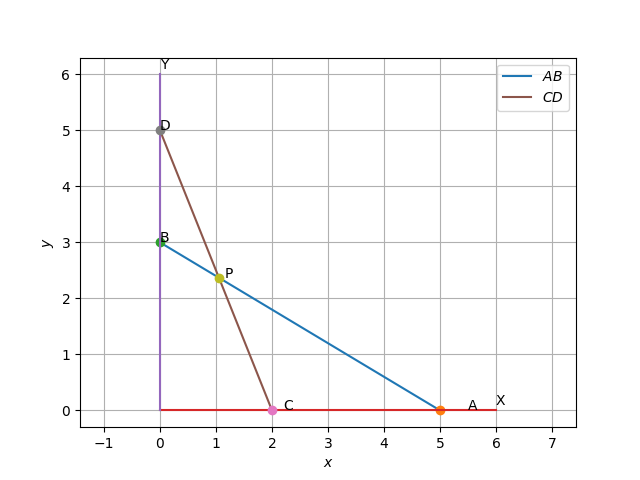
\includegraphics[width=\columnwidth]{Figure_1.png}
\caption{optimal point through the intersection of various lines}
\label{fig:Figure_1}
\end{figure}\\
The given problem can be expressed in general as matrix inequality as:
\begin{align}
\max_{\vec{x}} Z &= \myvec{5 & 3}\vec{x}
\\
s.t. \quad 
\myvec{
3 & 5
\\
5 & 2
}
\vec{x} &\preceq \myvec{15\\10}
\\
\vec{x} &\succeq \vec{0}\\
\vec{y} &\succeq \vec{0}
\end{align}
\begin{align}
\max_{\vec{x}} &\vec{c}^{T}\vec{x}
\\
s.t. \quad \vec{A}\vec{x} &\le \vec{b},
\\
\vec{x} &\succeq\vec{0}\\
\vec{y} &\succeq \vec{0}
\end{align}
%
where
\begin{align}
\vec{c} &= \myvec{5 \\ 3}
\\
\vec{A} &=
\myvec{
3 & 5
\\
5 & 2
}
\\
\vec{b}&=\myvec{15\\10}
%
\end{align}
%
and can be solved using {\em cvxpy} through the following code
\begin{lstlisting}
code/Assignment_3.py
\end{lstlisting}
Hence,
\begin{align}
\vec{x} = \myvec{1.05263158\\2.36842105}, Z = 12.36842102
\end{align}

\end{document}